\documentclass[8pt]{beamer}
%\usepackage{comment}
\usepackage{style}
\title[ Proyecto Junior PIJ-15-19]{  Estudio de la distribución de hidrógeno fotoionizado en el Centro Galáctico }
\author[Dr. Ericson López, Jr. Jairo Armijos, et. al.]{\large	 Dr. Ericson López, Jr. Jairo Armijos, et. al. \\ \vspace{0.2cm}
GRUPO DE RADIOASTRONOMÍA \\ \vspace{0.2cm} DEL OBSERVATORIO ASTRON\'OMICO DE QUITO}
\date{Quito, noviembre 2019.}
\begin{document}
\begin{frame}
\rule[0.05mm]{162mm}{0.05mm}
\begin{minipage}[d]{30mm}
\begin{center}

\includegraphics[scale=.20]{logo_epn.eps}
\end{center}
\end{minipage}
\begin{minipage}[d]{60mm}
\begin{center}
\vspace{0.2cm}
\textsf{\textbf{ ESCUELA POLIT\'ECNICA NACIONAL }}\\
\textsf{\textbf{ \small OBSERVATORIO ASTRON\'OMICO DE QUITO }}
%\textsf{\textbf{\tiny  Grupo de Cosmolog\'ia y Relatividad General}}\\
\end{center}
\end{minipage}
\begin{minipage}[d]{30mm}
\begin{center}

\includegraphics[scale=.55]{oaq.png}
\end{center}
\end{minipage}\\
\rule[1mm]{162mm}{0.20mm}
\maketitle
\end{frame}
\begin{frame}
\tableofcontents
\end{frame}
\begin{frame}
\frametitle{Campos magnéticos en las afueras de  galaxias}
\section{Campos magnéticos en las afueras de  galaxias}
\textbf{\big Resumen:}\\
Utilizando datos públicos de monóxido de carbono(CO), se estudiaron las condiciones de excitación del CO y la intensidad de campo magnético de  cuatro galaxias espirales. 
\begin{comment}
Para las afueras de las galaxias se encontraron temperaturas cinéticas $\lesssim 35-38K$, densidades de columna de CO $\lesssim 10^{15}-10^{16}cm^{-2}$, y masas de hidrógeno molecular $H_2$ $\lesssim 4\times 10^{6}-6\times10^{8}M_{\odot} $. La intensidad de campo magnético estimada es $\lesssim 6-31 \mu G$ 
\end{comment}
\end{frame}
\begin{frame}
\frametitle{Metodología}
Para el estudio del campo magnético en las afueras de las cuatro galaxias espirales, se utiliza el método de Dotson[1] que permite obtener una ecuación magnetohidrodinámica simplificada. Esta ecuación permite hallar un límite superior de la intensidad de campo magnético $B$:
\begin{equation*}
    B<3.23\times 10^{-8}\left(\frac{R}{pc}\right)^{0.5}\left(\frac{n}{cm^{-3}}\right)^{0.5}\left(\frac{M}{M_{\odot }}\right)^{0.5}\left(\frac{r}{pc}\right)^{-1}
\end{equation*}
donde $R$ es el radio de las líneas de campo magnético, $n$ la densidad del hidrógeno molecular, $M$ y $r$ la masa total y el radio de la galaxia. Los datos utilizados corresponden a mediciones de CO(2-1) obtenidas con el telescopio IRAM 30m a una frecuencia de $230GHz$ y una resolución espacial de 13 segundos de arco.
\begin{center}
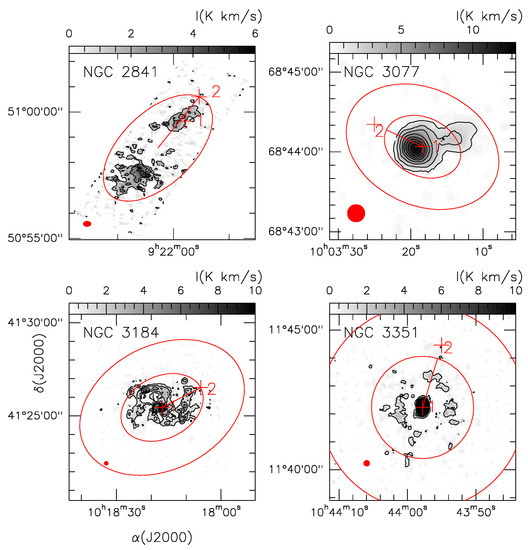
\includegraphics[width=0.8\linewidth]{figures/galaxies.jpg}
\captionof{figure}{Mapa de intensidad integrada de CO(2-1) de las cuatro galaxias estudiadas }
\end{center}
\end{frame}
\begin{frame}
\frametitle{Resultados: }
\textbf{Masa de la Galaxia}:  La masa de hidrógeno $M_{H_2}$ para la galaxia y sus afueras se derivó usando la expresión
\begin{equation*}
    \dfrac{M_{H_2}}{M_{\odot}}=5.5\dfrac{R_{21}}{0.8}\left(\dfrac{L_{CO}}{Kkms^{-1}pc^2}\right)
\end{equation*}
donde $R_{21}$ es un cociente de intensidad de línea $CO(2-1)/CO(1-0)$ y $L_{CO}$ es la luminosidad de CO[2].
Se encontró que la masa en las afueras de las galaxias son $\lesssim 4\times10^{6}-1\times10^{9}$ masas solares.\\

\textbf{Campo magnético en las galaxias y sus afueras}


\begin{center}
\begin{tabular}{ c c c } 
\hline
Galaxia& Región & B$(\mu G)$\\
 \hline
 NGC2841 & Disco & $\lesssim31$ \\
  & Afueras & ... \\
\hline
 NGC3077 & Disco & $\lesssim 6$ \\ 
   & Afueras & $\lesssim 7$ \\
 \hline
 NGC3184 & Disco & $\lesssim 14$ \\
   & Afueras & $\lesssim 19$ \\
\hline
 NGC3351 & Disco & $\lesssim 11$ \\
   & Afueras & $\lesssim 15$ \\

 \hline
\end{tabular}
\end{center}
}
\end{frame}
\begin{comment}
\begin{frame}
\frametitle{Conclusiones}
\begin{itemize}
    \item La intensidad de campo magnético estimada es $\lesssim 6-31\mu G$ que son consistentes con aquellas de  $\sim 20-60\mu G$ observadas en galaxias espirales.
    %Este resultado sugiere que el polvo es la principal componente que influencia el campo magnético en comparación con el gas molecular.
    \item En las afueras de las galaxias, la temperatura cinética es $\lesssim 35-38K$, la densidad de columna  de CO$\lesssim 10^{15}-10^{16}cm^{-2}$, la masa $M_{H_2}$ $\lesssim4\times10^6-6\times 10^{8}$ masas solares y la densidad de hidrógeno $\lesssim10^3cm^{-3}$.
    
\end{itemize}
\end{frame}
\begin{frame}
\frametitle{Cinemática y Masa de la Galaxia NGC7331}
\textbf{\big Resumen:}\\
e llevó a cabo un estudio de la curva de rotación de la galaxia NGC 7331, usando observaciones radioastronómicas del monóxido de carbono (CO). La forma de
la curva de rotación y las velocidades son similares a las derivadas previamente, empleando datos de hidrógeno atómico, esto sugiere la coexistencia de ambos elementos en las regiones estudiadas en NGC 7331. Asimismo, se estudió el campo de velocidades, lo que puso en
evidencia la rotación de la galaxia en sentido horario. Finalmente, se estimó una masa dinámica de 1,4E+10 masas solares para NGC 7331. 
\end{frame}
\begin{frame}
\frametitle{Análisis de datos}
NGC 7331 es una galaxia espiral cercana, situada a 14.7 Mpc de la Tierra[1]. Los datos de CO (2-1) se obtuvieron con el radio
telescopio IRAM de 30 metros de diámetro, a 230.5GHz y una resolución espacial de 13 segundos de arco. \\
\textbf{ MAPA Y ESPECTROS DE LA GALAXIA NGC 7331 }
\begin{center}
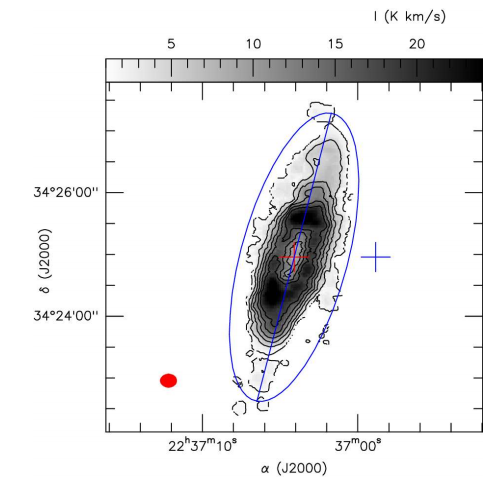
\includegraphics[width=0.58\linewidth]{ngc7331_1.png}
\captionof{figure}{\footnotesize{Mapa de intensidad integrada de CO (2-1) de NGC 7331.}   }
\end{center}

\begin{multicols}{2}
\begin{center}
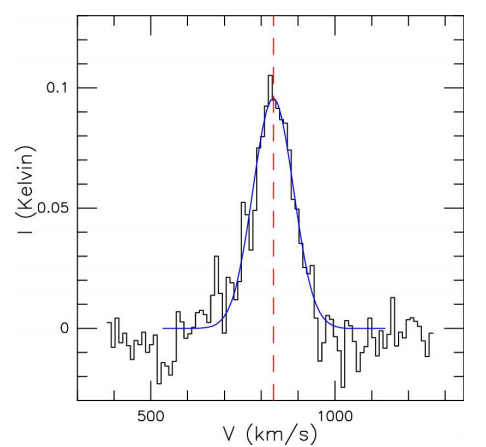
\includegraphics[width=0.96\linewidth]{ngc2.png}
\captionof{figure}{ \footnotesize{Espectro de emisión de CO (2-1) del centro de NGC 7331.} }
\end{center}

\begin{center}
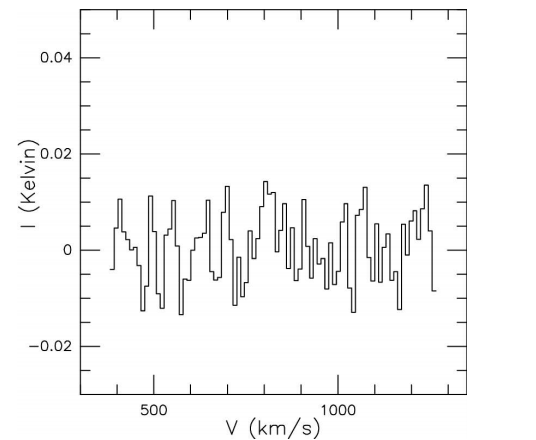
\includegraphics[width=0.98\linewidth]{ngc3.png}
\captionof{figure}{\footnotesize{Espectro observado en una posición alejada  del centro de NGC 7331. Indicada con una cruz azul en el mapa.}}
\end{center}	

\end{multicols}
\end{frame}
\begin{frame}
\frametitle{Resultados}
\textbf{CURVA DE ROTACIÓN}\\
Una curva de rotación muestra la velocidad del gas en función de una posición. La curva de rotación de NGC7331 se muestra abajo.
\begin{center}
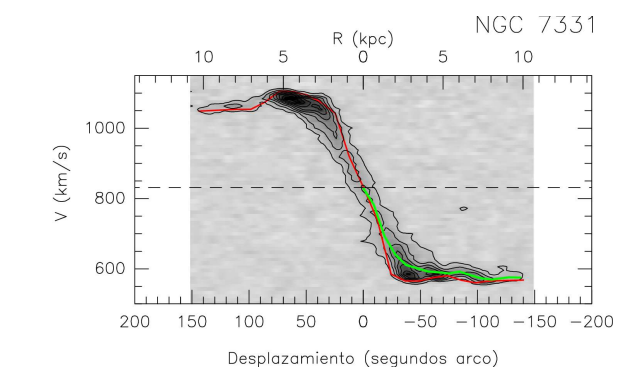
\includegraphics[width=0.75\linewidth]{rotacion.png}
\captionof{figure}{Diagrama donde se muestra la velocidad del gas en función de la posición en la galaxia. Las líneas rojas y verdes representan velocidades de rotación.}
\end{center}
}

Conclusiones 
\begin{itemize}
    \item La forma de la curva de rotación y las velocidades de NGC 7331 derivadas a partir de observaciones de la transición CO (2-1) son muy similares a aquellas
derivadas usando el hidrógeno atómico[2]. Este
resultado sugiere la coexistencia del gas de monóxido de
carbono e hidrógeno atómico en las regiones estudiadas.
\item El campo de velocidades del CO muestra que la galaxia NGC 7331  rota en sentido horario. 
\item Usando una aproximación esférica para la forma de la galaxia, se deriva una masa dinámica de 1,4E+10 masas solares para la galaxia NGC 7331. 

\end{itemize}
\end{frame}
\end{comment}
\end{document}